\documentclass[10pt,sigconf,nonacm]{acmart}
\usepackage{booktabs}
\usepackage{graphicx}
\usepackage{xspace}
\usepackage{amsmath}
\usepackage{tikz}
\usetikzlibrary{arrows.meta,positioning}
\emergencystretch=1em
\setcopyright{none}
\settopmatter{printacmref=false,printfolios=true}
\renewcommand\footnotetextcopyrightpermission[1]{}
\newcommand{\sysname}{BrowseTrace\xspace}
\newcommand{\mib}{\,MiB\xspace}
\newcommand{\artifacturl}{\url{https://github.com/landigf/publication-artifacts/tree/main/BrowseTrace}}
% Generated from released inputs; do not edit.
\newcommand{\BTCorpusAttempts}{1,311}
\newcommand{\BTScriptedAttempts}{400}
\newcommand{\BTLLMAttempts}{911}
\newcommand{\BTLLMPositive}{813}
\newcommand{\BTLLMEmpty}{98}
\newcommand{\BTScriptedRecorded}{168,067}
\newcommand{\BTLLMRecorded}{357,782}
\newcommand{\BTScriptedMean}{420.2}
\newcommand{\BTLLMMean}{392.7}
\newcommand{\BTLLMPositiveMean}{440.1}
\newcommand{\BTOverallRatio}{0.935}
\newcommand{\BTPositiveRatio}{1.047}
\newcommand{\BTScriptedLiveness}{357}
\newcommand{\BTLLMLiveness}{723}
\newcommand{\BTScriptedLivenessPct}{89.2}
\newcommand{\BTLLMLivenessPct}{79.4}
\newcommand{\BTLLMPositiveLivenessPct}{88.9}
\newcommand{\BTScriptedReplay}{82,455}
\newcommand{\BTScriptedZeroSize}{0}
\newcommand{\BTLLMReplay}{236,073}
\newcommand{\BTLLMZeroSize}{121,709}
\newcommand{\BTScriptedLRURequestPct}{37.4}
\newcommand{\BTScriptedLRUBytePct}{24.9}
\newcommand{\BTScriptedGDSFRequestPct}{59.5}
\newcommand{\BTScriptedGDSFBytePct}{15.8}
\newcommand{\BTLLMLRURequestPct}{43.5}
\newcommand{\BTLLMLRUBytePct}{20.2}
\newcommand{\BTLLMGDSFRequestPct}{76.2}
\newcommand{\BTLLMGDSFBytePct}{24.7}
\newcommand{\BTScriptedPositiveKeys}{17,144}
\newcommand{\BTScriptedVaryingKeys}{3,136}
\newcommand{\BTLLMPositiveKeys}{17,931}
\newcommand{\BTLLMVaryingKeys}{5,637}


\begin{document}
\title{BrowseTrace: Reproducible HTTP Traces and Cache Replay for Browser-Mediated AI Workloads}
\author{Gennaro Francesco Landi}
\affiliation{\institution{ETH Zurich}\city{Zurich}\country{Switzerland}}
\date{6 October 2026}
\renewcommand{\shortauthors}{G. F. Landi}
\keywords{browser agents, HTTP traces, workload measurement, cache replay, reproducibility}

\begin{abstract}
Browser agents generate sequences of web requests while executing natural-language tasks. Evaluating their network footprint requires distinguishing collected attempts, traffic-producing sessions, and the requests retained for replay. We present \sysname, a sanitized trace artifact and an empirical study of browser workloads across ten task families. Its session census covers 400 scripted sessions and 911 LLM-driven attempts across six model labels; 813 LLM attempts produce recorded traffic. A separate 300-attempt local comparison produces 3.3--4.2 times the mean request count of the local scripted driver. The pooled main corpus instead gives a ratio of 0.94 over all LLM attempts and 1.05 over traffic-producing attempts, demonstrating that the local comparison does not establish a general amplification factor. We replay 82{,}455 scripted and 236{,}073 positive-size LLM records using six cache policies at five capacities. At 5\mib, GDSF raises scripted request hits from \BTScriptedLRURequestPct\% to \BTScriptedGDSFRequestPct\% relative to LRU while reducing byte hits from \BTScriptedLRUBytePct\% to \BTScriptedGDSFBytePct\%. The released census, opaque-key traces, generated tables, and pinned replay environment make these descriptive findings reproducible offline. The study does not measure task success, estimate production traffic, or model HTTP cache correctness.
\end{abstract}
\maketitle
\hypersetup{pdfauthor={Gennaro Francesco Landi},pdfsubject={Research preprint, 6 October 2026; not peer reviewed}}
\pagestyle{plain}
\raggedbottom
\noindent\textit{Preprint, 6 October 2026. This version has not undergone peer review.}

\section{Introduction}
\label{sec:intro}
When a browser agent compares cloud services or searches technical documentation, the browser issues more than the navigation requests named by the agent. It fetches scripts, stylesheets, images, and other resources selected by the visited pages. The resulting request stream is a systems workload in its own right. A task-level score cannot identify its object reuse, transfer volume, or sensitivity to an eviction policy. Conversely, a small request count cannot establish that the agent answered the task correctly.

Existing web-agent research supplies useful task and interaction benchmarks. WebArena evaluates functional task completion in a reproducible web environment~\cite{webarena}; WebVoyager studies agents operating on real websites~\cite{webvoyager}. Our question is complementary: \emph{what can a reproducible request-level artifact establish about the measured browser workloads and their object-cache replay?} Answering it requires explicit accounting. An attempted session with no observed requests differs from a traffic-producing session. A positive recorded response size differs from HTTP cacheability. A local comparison with one driver differs from a representative estimate of agent traffic.

\sysname contributes a collection substrate and an artifact organized around these distinctions. The main census contains 1{,}311 collected attempts: 400 scripted and 911 LLM-driven. It preserves the 98 zero-request LLM attempts rather than silently dropping them. A separate local comparison contains 300 LLM attempts and uses the 100-session Zurich subset of the scripted corpus as its reference. A ten-task record from one human participant is retained solely to document the artifact's scope. It supplies no human population baseline.

The measurements support two main findings. First, the magnitude of a traffic comparison depends strongly on its cohort and denominator. The three model labels in the separate local comparison produce 3.3--4.2 times as many recorded requests per attempt as the local scripted reference. Pooling the main corpus instead gives approximately equal mean request counts, with the ratio changing from 0.94 to 1.05 when empty LLM attempts are excluded. These are descriptions of different collection designs, not competing estimates of one causal effect. Second, request and byte hit rates can favor different eviction policies. At 5\mib on the scripted replay, GDSF produces 22.1 percentage points more request hits than LRU but 9.1 percentage points fewer byte hits. Reporting request hits alone would obscure this tradeoff.

The contribution is a bounded empirical artifact rather than a task-success leaderboard or a new eviction algorithm:
\begin{enumerate}
\item A sanitized session census that separates the main corpus, local comparison, and single-participant record, including positive and empty attempts.
\item A cohort-specific traffic characterization that makes the denominator and collection differences explicit.
\item A reproducible replay of two fixed object streams, with both request and byte hit rates and a bijective sanitization of object identities.
\end{enumerate}
The accompanying publication package contains the inputs and generators for every retained numerical result. Its object-cache model deliberately omits HTTP freshness, authorization, and representation validation. Those omissions limit its interpretation to replay of the released objects.

\section{Collection substrate and task design}
\label{sec:collection}
\subsection{Tasks and two execution modes}
The collector uses Browser Use~\cite{browseruse} to control a headless Chromium browser on publicly reachable web pages. Ten task specifications cover news aggregation, cloud GPU comparison, literature search, fact checking, travel planning, regulatory lookup, job search, apartment comparison, weather API comparison, and documentation lookup. Table~\ref{tab:tasks} gives their concrete descriptions. These tasks were selected to exercise varied sites and navigation patterns; they are not a sample drawn from a distribution of deployed agent tasks.

\begin{table}[t]
\centering\small
\caption{Task specifications supplied to the collector. These describe requested work; the corpus does not contain validated completion labels.}
\label{tab:tasks}
\begin{tabular}{@{}p{0.27\columnwidth}p{0.65\columnwidth}@{}}
\toprule
Task family & Requested work \\
\midrule
News & Summarize five important AI news stories from today. \\
Cloud GPUs & Compare pricing, specifications, and availability across AWS, GCP, and Azure. \\
Literature & Find ten recent papers on LLM web agents and summarize their contributions. \\
Fact checking & Verify whether the EU AI Act requires all AI systems to be registered in a public database. \\
Travel & Find flights, hotels, and attractions for a weekend in Zurich. \\
Regulatory & Find GDPR articles relevant to collecting AI training data. \\
Jobs & Find ten ML engineer positions in Zurich with salary information. \\
Apartments & Compare rents for two-bedroom apartments across Zurich districts. \\
Weather APIs & Compare five providers on pricing, rate limits, and data quality. \\
Documentation & Summarize asyncio event loops, tasks, coroutines, and synchronization primitives. \\
\bottomrule
\end{tabular}
\end{table}

In \emph{LLM-driven mode}, Browser Use supplies browser observations to the selected language model, which chooses actions. The retained runner disables vision, allows up to four actions per step, sets a 60-second step timeout and a failure limit of ten, and enables direct opening of URLs. The user task prompt contains its name, description, category, access-pattern label, and starting URLs. For example, the documentation task asks for the asyncio concepts in Table~\ref{tab:tasks} and starts at the Python asyncio documentation and the MDN Fetch API page. The shared instructions require staying with the target publishers except for redirects, avoiding login, account creation and payment, and stopping when a short answer can be returned. The access-pattern label is a prompt field, not an enforced policy for the LLM.

Stopping can therefore occur when the framework completes, reaches its step limit, or encounters failure. Framework completion is not a semantic success annotation. The main LLM census includes heterogeneous limits: the 100-attempt Zurich Docker GPT extension uses eight steps; one initial Qwen attempt uses ten; the remaining 810 attempts use twenty. The separate local comparison uses twenty steps. The scripted release uses a fifteen-navigation limit. These differences are part of the collection design and prevent attributing pooled differences solely to model choice.

In \emph{scripted-random mode}, a credential-free driver builds a navigation plan from the task's starting URLs and same-site links. The planning code uses the repeat index as a pseudorandom seed. It shuffles roots or discovered links according to the task's scripted access pattern and truncates the plan at the navigation limit. It retries each navigation at most once and waits one second after navigation. The plan-selection seed is reproducible; live pages, redirects, and network responses are not. This driver is a reference workload for replay and traffic description, with no mechanism for answering or validating the natural-language task.

The browser configuration restricts navigation to the configured domains and uses a study-specific user-agent string. Embedded resources can still come from third-party domains. Configured restrictions document intended execution behavior; the release does not certify that every original agent action complied with the prompt.

\subsection{Request capture and its boundaries}
Instrumentation subscribes to the Chrome DevTools Protocol (CDP) Network events \texttt{request\allowbreak Will\allowbreak Be\allowbreak Sent}, \texttt{response\allowbreak Received}, \texttt{loading\allowbreak Finished}, and \texttt{loading\allowbreak Failed}~\cite{cdp}. It attaches to the initial focused target and registers newly created or focused tabs. A pending record is populated with the URL, method, timestamp, response metadata, and available timing fields. Completion creates a trace record; export also flushes pending requests using their currently recorded size. The size field is derived from CDP's encoded-data-length reporting, rather than an independent packet capture or a measurement of decoded page content.

Throughout this paper, \emph{request count} means the number of emitted trace records. It is not guaranteed to equal every HTTP exchange made by the browser. The collector indexes pending records by CDP request ID and retains a redirect count; a redirect chain is not represented as a separately verified complete set of hops. Target attachment timing, worker traffic, request-ID handling across targets, browser-side caching, and incomplete requests can also affect capture. No independent packet-level completeness audit is available for the original runs. We consequently make no claim of a full browser waterfall or complete wire-byte measurement.

The typed schema includes timing, response headers, status, resource type, session identifier, and an object identity. The publication results require a smaller surface: sanitized session aggregates and the canonical object-replay CSVs. We exclude historical claims about protocol shares, resource composition, or provider-specific per-request behavior that cannot be recomputed from that public surface.

\subsection{Regions and historical provenance}
The scripted corpus has ten repeats of each task in four locations: Zurich, US Central, Europe West, and Asia Southeast. The LLM extension spans these locations plus Australia Southeast, South America East, and a Zurich cloud deployment. Provider and machine names in raw metadata are normalized into region labels in the sanitized census. Region labels such as \texttt{eu-west} and \texttt{europe-west1} identify corresponding collection locations; they are not additional independent regions.

The corpus combines collection bundles rather than one balanced factorial experiment. Model labels, regions, step budgets, and collection sources are unevenly represented. Browser and framework versions were not recorded consistently enough to reconstruct every original runtime exactly. The current collection code documents the retained orchestration, while the released census documents session accounting. The pinned environment in the publication package supports \emph{offline analysis and replay}; it does not turn historical live collection into a deterministic experiment.

\section{Artifact construction and accounting}
\label{sec:artifact}
\subsection{Three cohorts, three purposes}
The census assigns a collision-free artifact-local identifier to each attempt and records cohort, source, workload, model label, region, task, request count, byte count, and whether the request count is positive. It exports no original session identifiers, private paths, URL strings, or headers. The source field names a collection bundle, allowing aggregate checks without disclosing machine-specific paths.

\begin{table}[t]
\centering\small
\caption{Census accounting. The local LLM comparison and human record are separate from the main corpus. Its scripted reference is the already-counted 100-session Zurich subset.}
\label{tab:cohorts}
\setlength{\tabcolsep}{3pt}
\resizebox{\columnwidth}{!}{% Generated from released inputs; do not edit.
\begin{tabular}{lrrrr}
\toprule
Cohort & Attempts & Nonempty & Requests & Mean \\
\midrule
Scripted (main) & 400 & 400 & 168,067 & 420.2 \\
LLM (main) & 911 & 813 & 357,782 & 392.7 \\
LLM (local comparison) & 300 & 300 & 158,231 & 527.4 \\
Human (one participant) & 10 & 10 & 5,282 & 528.2 \\
\bottomrule
\end{tabular}
}
\end{table}

The \emph{main corpus} contains 400 scripted sessions and 911 LLM attempts. All scripted sessions and 813 LLM attempts have at least one trace record, giving 1{,}213 traffic-producing sessions. The remaining 98 attempts are empty. Their presence does not determine why a run failed to generate traffic: the released census alone cannot distinguish provider failure, browser failure, missing capture, or other causes.

The \emph{local comparison} contains a separate 300 LLM attempts: 150 Flash, 50 Pro, and 100 GPT-4.1-mini. Their reference is the 100-session scripted Zurich subset. These records are kept under a distinct cohort label and are not added to the headline 911 LLM attempts or the main LLM cache stream. The \emph{human record} has ten task-sessions from one participant. The complete census thus has 1{,}621 rows: 1{,}311 main-corpus attempts, 300 local-comparison attempts, and ten human task-sessions.

Model names in this paper are the normalized labels in collection metadata. The LLM replay CSV does not retain collision-free per-row model attribution. It uses legacy task-scoped session labels that repeat across models and regions. Counting unique labels in that CSV would give a false session count; joining those labels directly to the census would also be ambiguous. The census supports session-level counts by model. The released replay supports pooled object-cache experiments, not trustworthy per-model cache curves.

\subsection{A mechanical capture check}
An accompanying audit defines \emph{reached content} as at least three distinct URL hostnames and at least five HTTP-200 responses with a non-root path. The released per-attempt audit retains numeric counters and the boolean result, allowing the predicate and aggregate accounting to be checked without URL disclosure. It holds for 357 of 400 scripted sessions and 723 LLM attempts. The LLM percentage is 79.4\% over all 911 attempts or 88.9\% over the 813 traffic-producing attempts. In the separate local comparison, 274 of 300 attempts satisfy the predicate.

This predicate is a liveness heuristic. Third-party resources can contribute hostnames and non-root successes without completing the requested task. A successful documentation lookup can conversely stay within fewer than three hosts. It should therefore be used to expose a capture property, not to filter the corpus into alleged successful tasks. The public counters permit re-evaluating the published predicate; recomputing those counters from scratch requires the unreleased raw requests.

\subsection{Canonical replay inputs and sanitization}
The main scripted census accounts for \BTScriptedRecorded{} recorded requests; its pinned replay input contains \BTScriptedReplay{} positive-size records. An audit of the complete historical scripted JSON confirms the census counts and byte totals. Its positive-size count, size multiset, and timestamp--size pair multiset agree with the replay input; the other 85{,}612 records have zero size. The LLM input retains all \BTLLMRecorded{} census records, with \BTLLMReplay{} positive-size and \BTLLMZeroSize{} zero-size rows. Scripted zero-size records were omitted before export, whereas LLM zero-size records are skipped during replay. Neither positive size nor this filtering establishes HTTP cacheability. The released projection audit contains aggregate counts and multiset digests; it does not reconstruct original row identities, keys, or stitching order.

The LLM filename \texttt{llm\_full\_901.csv} is retained for compatibility and does not describe its number of attempts. The publication manifest records actual row counts and checksums instead of relying on filenames. Each replay row contains a timestamp, cache key, object size, and legacy session label. The scripted file additionally contains an agent-type label. Replay consumes the stored row order; timestamps do not implement pacing, expiry, or concurrency. This order defines the experiment, without establishing a production interleaving of simultaneous clients.

For the publication package, all cache keys are replaced by opaque artifact-local tokens. Let $k_i$ be the original key of row $i$ and $f$ its released mapping. The sanitization check requires
\begin{equation}
f(k_i)=f(k_j) \quad\Longleftrightarrow\quad k_i=k_j
\label{eq:bijection}
\end{equation}
across both released streams. Row order, timestamps, sizes, and agent-type labels are preserved. Legacy session labels are separately remapped into artifact-local tokens while retaining their existing collisions; they still cannot identify individual model runs. Since the replay policies use identity equality and object size rather than URL semantics, this transformation preserves their inputs to eviction decisions. An equality check and replay comparison are included in the package.

Ordinary query redaction can merge distinct URLs into one key and change hit rates. Accordingly, the canonical opaque-key CSVs are the replay source of truth. They cannot be reconstructed by concatenating older uniformly redacted per-task exports. The original collector's URL-to-key policy also differs across retained code and historical inputs; our reproducibility claim begins with the pinned canonical streams rather than an inferred uniform key policy. Opaque identities prevent URL-based analyses and do not hide aggregate behavioral patterns; the release makes no formal anonymization guarantee.

\begin{figure}[t]
\centering
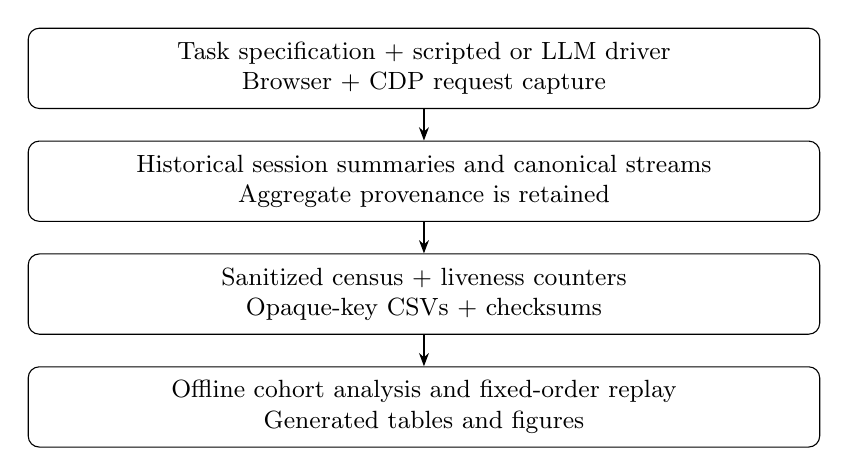
\begin{tikzpicture}[font=\small, node distance=4mm,
 box/.style={draw,rounded corners,align=center,text width=0.80\columnwidth,inner sep=5pt},
 >={Stealth}]
\node[box] (collect) {Task specification + scripted or LLM driver\\Browser + CDP request capture};
\node[box,below=of collect] (historical) {Historical session summaries and canonical streams\\Aggregate provenance is retained};
\node[box,below=of historical] (release) {Sanitized census + liveness counters\\Opaque-key CSVs + checksums};
\node[box,below=of release] (analysis) {Offline cohort analysis and fixed-order replay\\Generated tables and figures};
\draw[->] (collect)--(historical);
\draw[->] (historical)--(release);
\draw[->] (release)--(analysis);
\end{tikzpicture}
\Description{Four stacked stages connect browser task collection, historical summaries and streams, sanitized artifacts, and offline analysis with arrows.}
\caption{Publication data flow. Offline results are reproduced from the sanitized layer. Recreating historical live collection additionally needs original execution environments and mutable websites.}
\label{fig:pipeline}
\end{figure}

\section{Traffic measurements}
\label{sec:traffic}
\subsection{Main-corpus counts and empty attempts}
Table~\ref{tab:models} reports the main LLM census by model label. The corpus contains 357{,}782 recorded requests. GPT-4.1-mini contributes 350 attempts and 168{,}136 requests, while the five other labels contribute fewer attempts and uneven request totals. Pro has 86 zero-request attempts out of 150; GPT has two out of 350; Qwen has ten out of 61. The remaining labels have no zero-request attempts in the census. These differences affect any per-attempt statistic even before comparing navigation behavior.

\begin{table*}[t]
\centering\small
\caption{Main LLM corpus from the sanitized census. Empty attempts remain in the denominator for requests per attempt. Positive sessions have at least one emitted trace record.}
\label{tab:models}
% Generated from released inputs; do not edit.
\begin{tabular}{lrrrrrr}
\toprule
Model & Attempts & Nonempty & Empty & Mean & Median & Liveness \\
\midrule
claude-haiku-4.5 & 100 & 100 & 0 & 206.9 & 159.0 & 86/100 \\
deepseek-v3.2 & 100 & 100 & 0 & 385.1 & 315.0 & 85/100 \\
gemini-2.5-flash & 150 & 150 & 0 & 461.8 & 343.0 & 146/150 \\
gemini-2.5-pro & 150 & 64 & 86 & 321.9 & 0.0 & 47/150 \\
gpt-4.1-mini & 350 & 348 & 2 & 480.4 & 373.0 & 313/350 \\
qwen-2.5-coder-7b & 61 & 51 & 10 & 211.3 & 155.0 & 46/61 \\
\bottomrule
\end{tabular}

\end{table*}

\begin{figure}[t]
\centering
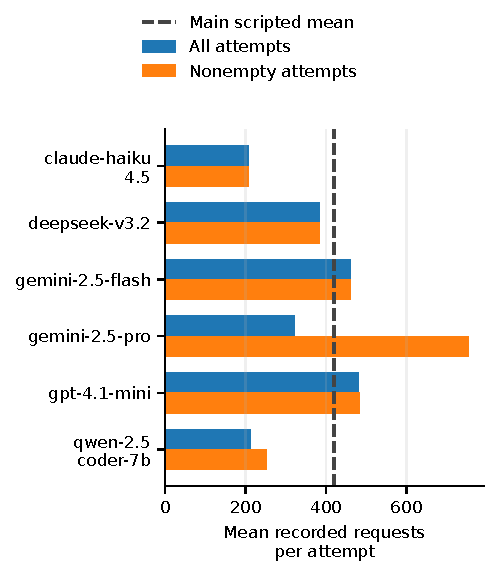
\includegraphics[width=\columnwidth]{figures/model-request-counts.pdf}
\Description{Paired bars for six model labels compare average recorded requests over all attempts and over nonempty attempts.}
\caption{Main-corpus mean recorded requests with all-attempt and positive-only denominators. Cohorts differ in region mix and step limits; these bars are descriptive, not a model-quality ranking.}
\label{fig:modelmeans}
\end{figure}

Over all \BTLLMAttempts{} main-corpus LLM attempts, the mean is \BTLLMMean{} requests. Restricting the same request total to the \BTLLMPositive{} positive attempts raises it to \BTLLMPositiveMean{}. The \BTScriptedAttempts{} scripted attempts have a mean of \BTScriptedMean{}. The respective LLM-to-scripted ratios are \BTOverallRatio{} and \BTPositiveRatio{}. Neither ratio establishes that the two modes perform equivalent useful work. They pool different location mixes, step budgets, and failure patterns. They do establish that the artifact does not support a universal three- or four-fold increase in per-session traffic.

\subsection{The separate local comparison}
Table~\ref{tab:local} retains a more narrowly specified comparison: LLM and scripted runs collected locally in Zurich over the same ten task definitions. The scripted reference generates 14{,}833 requests in 100 attempts, or 148.33 per attempt. Flash, Pro, and GPT generate 73{,}963, 30{,}898, and 53{,}370 requests in 150, 50, and 100 attempts, respectively. The corresponding means are 493.09, 617.96, and 533.70, giving ratios of 3.324, 4.166, and 3.598.

\begin{table}[t]
\centering\small
\caption{Separate local comparison. Ratios divide requests per LLM attempt by requests per scripted Zurich attempt. Counts are not added to the main LLM corpus.}
\label{tab:local}
% Generated from released inputs; do not edit.
\begin{tabular}{lrrr}
\toprule
Local cohort & Attempts & Mean requests & Ratio \\
\midrule
Scripted Zurich & 100 & 148.3 & 1.000 \\
gemini-2.5-flash & 150 & 493.1 & 3.324 \\
gemini-2.5-pro & 50 & 618.0 & 4.166 \\
gpt-4.1-mini & 100 & 533.7 & 3.598 \\
\bottomrule
\end{tabular}

\end{table}

\begin{figure}[t]
\centering
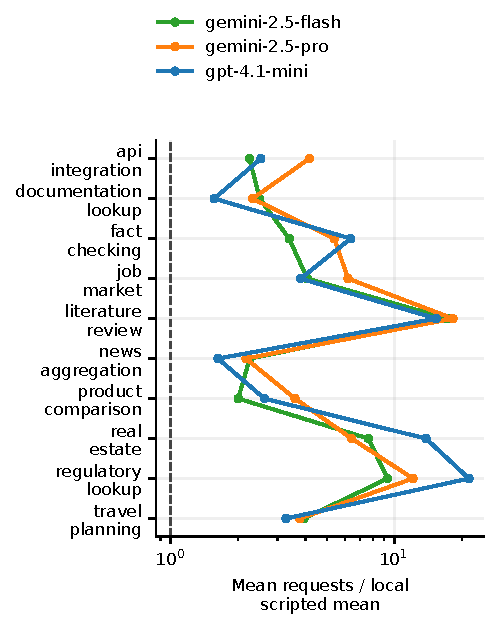
\includegraphics[width=\columnwidth]{figures/task-amplification.pdf}
\Description{Three series show model-to-scripted mean request ratios separately for each of ten task definitions in the local comparison cohort.}
\caption{Task-specific ratios in the separate local comparison. Each mean uses the cohort's number of attempts for that task; unequal model sample counts are not treated as equal totals. The scripted reference does not solve the requested task.}
\label{fig:taskratio}
\end{figure}

This local comparison shares task descriptions and a browser substrate, but it still compares different navigation policies and limits. LLM attempts have up to twenty decision steps with up to four actions per step, while scripted plans have a fifteen-navigation limit and a fixed post-navigation wait. The number of completed navigations, useful information obtained, and task success are not matched. A ratio is therefore a description of the specified executions, not the causal cost of adding an LLM to an otherwise identical workflow.

Task-specific ratios in Figure~\ref{fig:taskratio} further discourage using a single multiplier. They compare per-attempt means rather than raw task totals, because Flash has fifteen repeats per task, Pro five, and GPT ten. Constrained or blocked scripted navigation can create a small denominator even where an LLM run does not accomplish the task. We retain the ratios to make those workload differences inspectable, without labeling them network efficiency.

\subsection{Why the denominator matters}
The local scripted mean of 148.33 differs markedly from the four-location scripted mean of 420.17. Its 100 sessions are a subset, not an independent representative sample of a stable scripted traffic process. Dynamic site responses, collection location, and source bundle can all change emitted records. The local ratios and pooled ratios address different questions; neither should be generalized by selecting whichever ratio is larger.

The human record has 5{,}282 requests across ten tasks, with mean 528.2 and range 15--1{,}929. These ten sessions share a participant and cannot be treated as ten independent people. There is no matched task-success comparison or repeated participant sample. We include the counts for transparency and make no agent-to-human ratio claim.

The traffic results are census summaries of this release. We do not report a population confidence interval from the combined corpus: its attempts were not independently sampled from a defined deployed-workload distribution, and model-by-region coverage is uneven. The plots show measured averages without error bars. The corpus supports exact recomputation of those averages and denominators; broader inference needs a new sampling and task-validation design.

\section{Offline object-cache replay}
\label{sec:replay}
\subsection{Model and reference implementation}
Replay evaluates the released sequence of $(k_i,s_i)$ pairs, where $k_i$ is an opaque identity and $s_i$ the recorded object size. Each configuration starts with an empty cache and processes one complete fixed stream in stored order, without warmup exclusion. On a miss, an incoming object larger than the capacity is not admitted. The experiment covers capacities of 1, 5, 10, 25, and 50\mib and six policies: LRU, LFU, ARC~\cite{arc}, S3-FIFO~\cite{s3fifo}, W-TinyLFU~\cite{tinylfu}, and GDSF~\cite{gdsf}. Their reference implementations are those in the pinned \texttt{libcachesim==0.3.3.post4} Python package~\cite{libcachesim}, with its release defaults. We do not use the older custom Python simulator as the numerical authority.

The pinned library's CSV reader skips zero-size records during trace processing, making the effective denominators \BTScriptedReplay{} for scripted and \BTLLMReplay{} for LLM. LLM zero-size rows remain in the trace file and census accounting. Their exclusion here does not prove that they correspond to network failures or that they are irrelevant to a different request-cost model.

For hit indicator $h_i\in\{0,1\}$, we report
\begin{equation}
H_{\mathrm{req}}=\frac{\sum_i h_i}{N},\qquad
H_{\mathrm{byte}}=\frac{\sum_i h_i s_i}{\sum_i s_i}.
\label{eq:rates}
\end{equation}
The byte metric weights a hit by the current record's size. Repeated keys do not establish equal representations: \BTScriptedVaryingKeys{} of \BTScriptedPositiveKeys{} distinct positive-size scripted keys and \BTLLMVaryingKeys{} of \BTLLMPositiveKeys{} LLM keys occur with more than one positive size. These keys account for 62{,}692 scripted and 212{,}857 LLM positive-size records. In the pinned library, a hit does not update the resident object's size accounting; a new admission uses the incoming size. A five-record check, $A(1),B(1),A(9),C(2),A(1)$, yields resident occupancy $1,2,2,4,4$ bytes for all six policies with ample capacity, even though the third record contributes nine hit bytes to the byte metric. The released model audit reproduces this behavior and the variable-size-key counts.

Capacity therefore bounds the sizes recorded at admission, with policy metadata excluded. It does not establish the space needed for valid physical HTTP representations or a total-process RAM budget. The runner uses the standard \texttt{process\_trace} path with admission and eviction, rather than an unconditional-insert path. We measure hit rates, not CPU cost, latency, concurrency, storage writes, or throughput. The sixty configurations are six policies times five capacities times two streams, not sixty independent samples. Repeating the same deterministic replay is a reproducibility check and creates no additional statistical trials.

\subsection{Results: request hits and byte hits diverge}
Table~\ref{tab:cache5} shows all six policies at 5\mib. On the scripted trace, GDSF has a \BTScriptedGDSFRequestPct\% request hit rate against LRU's \BTScriptedLRURequestPct\%, a gain of 22.1 percentage points. Byte hit rates go in the opposite direction: GDSF reaches \BTScriptedGDSFBytePct\% and LRU \BTScriptedLRUBytePct\%, a loss of 9.1 percentage points. The advantage in request hits therefore cannot be described as a corresponding reduction in transferred bytes.

\begin{table}[t]
\centering\small
\caption{Reference replay at 5\mib. Request and byte hit rates are percentages of positive-size records and their recorded bytes, respectively. The effective denominators are 82{,}455 scripted and 236{,}073 LLM records.}
\label{tab:cache5}
\setlength{\tabcolsep}{3pt}
\resizebox{\columnwidth}{!}{% Generated from released inputs; do not edit.
\begin{tabular}{lrrrr}
\toprule
Policy & Scripted request & Scripted byte & LLM request & LLM byte \\
\midrule
LRU & 37.4\% & 24.9\% & 43.5\% & 20.2\% \\
LFU & 27.3\% & 12.1\% & 50.3\% & 23.9\% \\
ARC & 36.2\% & 23.8\% & 46.1\% & 22.9\% \\
S3-FIFO & 42.4\% & 29.8\% & 55.5\% & 31.6\% \\
W-TinyLFU & 45.6\% & 11.8\% & 72.3\% & 24.2\% \\
GDSF & 59.5\% & 15.8\% & 76.2\% & 24.7\% \\
\bottomrule
\end{tabular}
}
\end{table}

The capacity curves in Figure~\ref{fig:cache} show the same distinction across the full sweep. GDSF prioritizes frequency relative to size, so retaining frequently requested small objects can improve the request-weighted metric while displacing larger objects that matter more to the byte-weighted metric. This mechanism is consistent with the observed tradeoff; the curves themselves establish only the result of the pinned replay. They do not identify which eviction policy a CDN or browser should deploy.

\begin{figure*}[t]
\centering
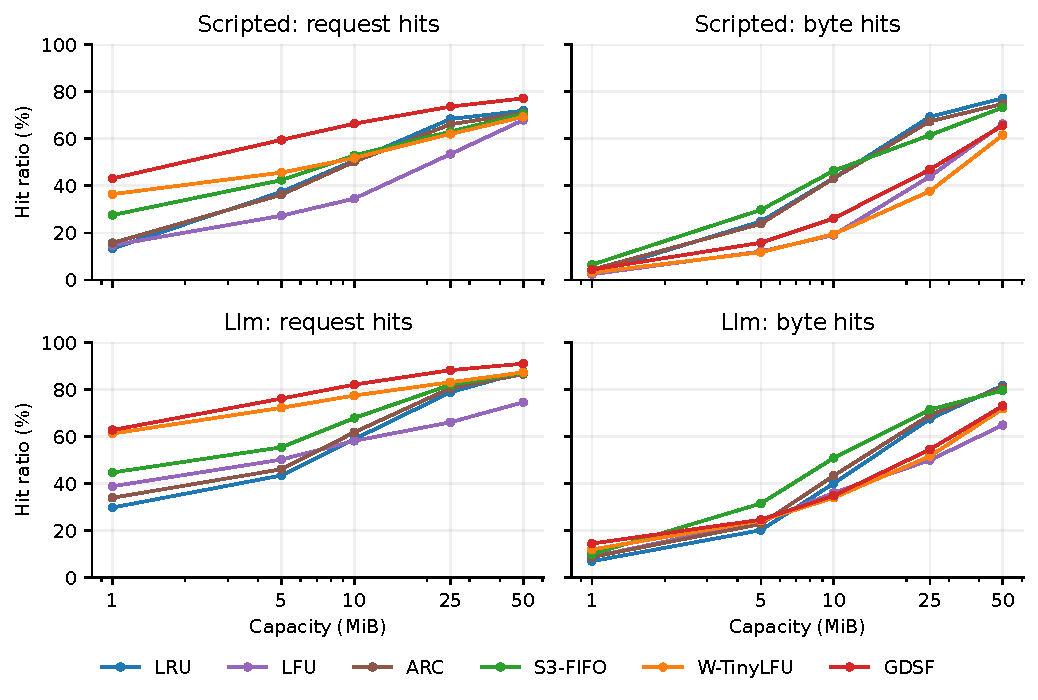
\includegraphics[width=\textwidth]{figures/cache-policy-tradeoff.pdf}
\Description{Four panels plot request and byte hit percentages versus cache capacity for scripted and LLM traces; six lines in each panel identify the six library policies.}
\caption{Cold-cache replay of the two fixed streams. Curves show request and byte hit rates at five capacities for the pinned library policies. There are no trial confidence intervals: each point is a complete deterministic evaluation of one released sequence. Both metrics are required to assess a policy's behavior.}
\label{fig:cache}
\end{figure*}

For the LLM stream, GDSF reaches \BTLLMGDSFRequestPct\% request hits and \BTLLMGDSFBytePct\% byte hits at 5\mib, against LRU's \BTLLMLRURequestPct\% and \BTLLMLRUBytePct\%. Here GDSF improves both metrics relative to LRU. Nevertheless, S3-FIFO has the highest byte hit rate among the six evaluated policies at that capacity on both streams, while GDSF has the highest request hit rate. The metric therefore changes the preferred policy even where GDSF improves both rates relative to LRU. The LLM stream's curves describe a different pooled object sequence and should be read separately from the scripted stream. Collection mix, sizes, repeated keys, and ordering can all affect the rankings. The curves do not isolate an intrinsic property of LLM agents, and the legacy labels do not support decomposition by individual model. A new dataset with collision-free request-level provenance would be needed for that experiment.

\subsection{Replay is not an HTTP cache}
An HTTP cache must consider freshness, method semantics, validators, authorization, and selected representations, including \texttt{Vary}~\cite{rfc9111}. Our replay uses identity equality and recorded size. It does not enforce \texttt{Cache-Control}, response eligibility, expiry, revalidation, method matching, privacy rules, or representation equivalence. An apparent repeated-key hit can therefore be invalid as an HTTP response reuse even though it is valid in the released object model.

The timestamps are retained, but replay does not derive expiry from HTTP freshness fields. All input records are offered to the simulated object cache regardless of whether a real shared cache could store their responses. Different responses sharing a legacy key may be counted as hits, and CDP sizes can reflect incomplete or already cached responses. Replay coverage must be calculated against census record counts: the scripted file already excludes zero-size rows, while the LLM file retains them. For these reasons, \emph{byte hits} means a simulated weighted-hit statistic, not measured bytes saved on a live network. No origin offload, CDN energy saving, or production capacity estimate follows from this study.

\section{Related work}
\label{sec:related}
WebArena~\cite{webarena} provides a controlled environment and functional task evaluation, while WebVoyager~\cite{webvoyager} evaluates browser agents on live website tasks. These establish the importance of specifying agent observations, tools, and completion criteria. \sysname instead exposes request counts and fixed object streams generated by a smaller collection of task definitions. It supplies no evidence that its agents are competitive on those benchmarks and makes no exhaustive claim that other agent datasets contain no network information.

Browser Use~\cite{browseruse} is the execution substrate, and CDP~\cite{cdp} supplies browser-network events. Our contribution is the measured corpus, its accounting, and the reproducible analysis layer, rather than these underlying interfaces. The distinction between recorded CDP events and complete HTTP exchanges matters for interpreting its request and size fields.

The evaluated eviction policies address different approaches to cache management. ARC adapts the balance between recency and frequency~\cite{arc}; TinyLFU supplies a frequency-based admission mechanism and W-TinyLFU combines it with a window~\cite{tinylfu}; S3-FIFO uses static FIFO queues and quick demotion~\cite{s3fifo}; GDSF incorporates size, access frequency, and recency~\cite{gdsf}. We use their library implementations~\cite{libcachesim} to characterize two workloads, without proposing algorithmic novelty or inferring superiority beyond those implementations and streams. RFC~9111~\cite{rfc9111} defines the HTTP semantics intentionally absent from the object replay.

\section{Limitations, ethics, and reproducibility}
\label{sec:limits}
\subsection{What can and cannot be learned}
The corpus supports exact cohort accounting, measured request-count summaries, predicate checks over released liveness counters, and fixed-stream object-cache replay. It does not support estimates of global agent traffic, validated task-cost efficiency, or per-model HTTP cache performance. Its ten task definitions, chosen sites, uneven model coverage, and heterogeneous limits provide a pilot workload collection. The live web and provider services changed during collection; a model label does not by itself identify an immutable model snapshot.

The retained runner and metadata explain the intended protocol. Missing runtime versions, complete action histories, task labels, and capture validation restrict reconstruction. Many subresources do not make the selected tasks representative, and a byte sum is not a validated traffic bill.

Release integrity has distinct layers: checksums identify the bytes, equality checks validate sanitization, and recomputation validates analysis. These checks do not certify unrecorded collection facts or supply missing per-row model attribution.

\subsection{Ethics and release boundary}
Task prompts forbid logging in, creating accounts, and making payments. The study uses browser access to public starting pages rather than private user accounts. These instructions reduce the intended interaction scope, but they are not a site-by-site authorization assessment or a complete audit of agent actions. The release makes no blanket assertion of compliance with every website's terms or robots policy. Offline reproduction sends no requests to the original publishers and requires no model API credentials.

Browser capture can include third-party tokens, headers, URL parameters, and content unrelated to the task. The publication package excludes raw HTTP header maps, URLs, and response bodies. Replay keys are replaced with opaque identities, and the census exposes aggregate numeric metadata. The older public repository's history is a separate exposure surface; this sanitized package does not certify that earlier commits are sanitized. Any repository-history cleanup and credential-owner decisions must be resolved before treating that history as a safe redistribution source. The publication archive is built from the reviewed file allowlist, not a complete repository export.

The ten single-participant sessions were performed by the author, who consented to publication of their aggregate counts. They expose no personal browsing profile and supply no human population inference. Authorship and release authority are recorded in the accompanying author-confirmation record; no institutional ethics-review approval is claimed.

\subsection{Reproducible package}
The accompanying artifact includes the sanitized census, per-attempt liveness counters, collection-metadata audit, opaque-key replay CSVs, environment specification, checksum manifest, result JSON, and table and plot generators. One offline command regenerates cohort summaries and all sixty cache configurations. The release check verifies row counts, positive-size denominators, nonnegative sizes, key relationships, and agreement between recomputed outputs and the manuscript inputs. Generated TeX tables are imported directly rather than copied into the paper by hand. The project repository is \artifacturl; the publication manifest identifies the exact checked files.

Existing code and data licenses are retained; a DOI is not claimed before deposit. Paper compilation and replay are independent. Live recollection requires external websites and model access and cannot reproduce historical responses deterministically. Raw bundles are needed to regenerate the census and liveness counters; published accounting is recomputed from the sanitized artifacts.

\subsection{AI assistance disclosure}
AI tools were used extensively for literature search, manuscript drafting and revision, analysis-code development, figure preparation, and automated technical and skeptical review. They did not create additional browser observations or validated task-success labels for this version. Retained numerical results are computed from the accompanying artifact and linked to generated reports. Automated review is not independent scholarly peer review. The named author remains responsible for approving the final manuscript, authorship, disclosures, and release rights.

\section{Conclusion}
\sysname makes a bounded browser-workload study reproducible through explicit cohort accounting and sanitized fixed-stream replay. The local three-model request ratios and pooled main-corpus ratios differ substantially because they describe different collection designs and denominators. At small capacities, a policy's request-hit advantage can coexist with a byte-hit disadvantage. These results motivate reporting the workload, denominator, identity model, and both hit metrics together. The released artifact provides a concrete basis for such evaluations while leaving task success, capture completeness, representative sampling, and HTTP-correct response reuse to future collection designs.

\label{sec:body-end}
\bibliographystyle{ACM-Reference-Format}
\bibliography{BrowseTrace-preprint}
\end{document}
